\begin{question}
 The reaction of the gaseous educt A with a dissolved educt B to product C is carried out in a isothermally operated batch reactor.
 %%
 \begin{equation*}
  \ch{A_g + B_{fl} -> C_{fl}}
 \end{equation*}
 %%
 The reaction rate $r$ was determined experimentally as a function of the concentration of B. The partial pressure of the gaseous educt A in the reactor was constant at \SI{1500}{\hecto\pascal} in all experiments. The Henry coefficient for A in the solvent is \SI{3.82e-3}{\milli\mole\per\liter\per\pascal}.
 %%
\renewcommand{\labelenumi}{\alph{enumi})}
\begin{enumerate}
\item Determine the rate constant $k$ and the value for $\beta_L * a$
\item What is the concentration of the gaseous educt A in the liquid under the respective reaction conditions? Calculate how large the concentration of A in the liquid is when no reaction takes place.
\item Compare the values of $\beta_L * a$ and $k * c_B$ for the highest stated concentration $c_B$. Is it possible to simplify the macrokinetic equation to determine the reaction rate $r$? Compare the given value $r$ with the value determined after simplification. 
\end{enumerate}
%%
The values for the concentration of B $c_{B,fl}$ and the reaction rate $r$ are given in Tab. \ref{tab8:1}.
\end{question}

\begin{pycode}
import numpy as np
import pandas as pd
import matplotlib.pyplot as plt
from sklearn.linear_model import LinearRegression
import tikzplotlib

pA = 1500e2 #Pa
Ha = 3.89e-6 #mol/(L*Pa)

cBfl = 1e-3*np.array([25, 150, 600, 1200, 4000, 6000]) # mol/L
r = 1e-6*1/60*np.array([27220, 94970, 151550, 168250, 182310, 184520]) #mol/(L*s)

# Creating a 2 dimensional numpy array
data = np.array([cBfl, r, 1/cBfl, 1/r])

# Creating pandas dataframe from numpy array
dataset = pd.DataFrame({'cB': data[0, :], 'r': data[1, :], '1overCb': data[2, :], '1overR': data[3, :]})
pd.DataFrame(dataset).to_csv("Tables/rateconc.csv", index=False, header=False)

X = dataset.iloc[:, 0].values.reshape(-1, 1)  # values converts it into a numpy array
Y = dataset.iloc[:, 1].values.reshape(-1, 1)  # -1 means that calculate the dimension of rows,

linear_regressor = LinearRegression()  # create object for the class
linear_regressor.fit(1/X, 1/Y)         # perform linear regression
Y_pred = linear_regressor.predict(1/X) # make predictions

intercept = linear_regressor.intercept_[0]
slope = linear_regressor.coef_[0,0]

k = 1/(slope*Ha*pA)
aBetaL = 1/(intercept*Ha*pA)
cAflwr = Ha * pA
\end{pycode}

\begin{solution}
The rate of such a type of reaction is defined by:
%%
\begin{equation}\label{eqn8:rate}
 r = k * H_A * \frac{a * \beta_L}{a * \beta_L + k * c_{B,fl}} * p_A * c_{B,fl}
\end{equation}
%%
Rearranging Eq. \ref{eqn8:rate} leads to:
%%
\begin{equation}
 \frac{1}{r} = \underbrace{\frac{1}{k * H_A * p_A}}_{\text{slope } m} * \frac{1}{c_{B,fl}} + \underbrace{\frac{1}{H_A * p_A * a * \beta_L}}_{\text{intercept } d}
\end{equation}
%%
The slope and intercept can be determined by a linear regression $r^{-1} = f\left(c_{B,fl}^{-1}\right)$.
%%
\begin{table}[H]
\centering
\caption{Given values and their reciprocal values}
\label{tab8:1}
\pgfplotstabletypeset[%
col sep=comma, header=false,
every head row/.style={before row={\toprule}, after row={\midrule}},
every last row/.style={after row=\bottomrule},
display columns/0/.style={column name={$\sfrac{c_{B,fl}}{\si{\mole\per\liter}}$}, string type, column type={S[table-format=1.3]}},
display columns/1/.style={column name={$\sfrac{r}{\si{\mole\per\liter\per\second}}$}, string type, column type={S[scientific-notation=true, round-precision=2, table-format=1.2e-1]}},
display columns/2/.style={column name={$\sfrac{c_{B,fl}^{-1}}{\si{\liter\per\mole}}$}, string type, column type={S[round-precision=2, table-format=2.2]}},
display columns/3/.style={column name={$\sfrac{r^{-1}}{\si{\liter\second\per\mole}}$}, string type, column type={S[round-precision=2, table-format=4.2]}},
]{Tables/rateconc.csv}
\end{table}
%%
\begin{center}
% This file was created by tikzplotlib v0.9.8.
\pgfkeys{/pgf/number format/.cd,1000 sep={\:}}
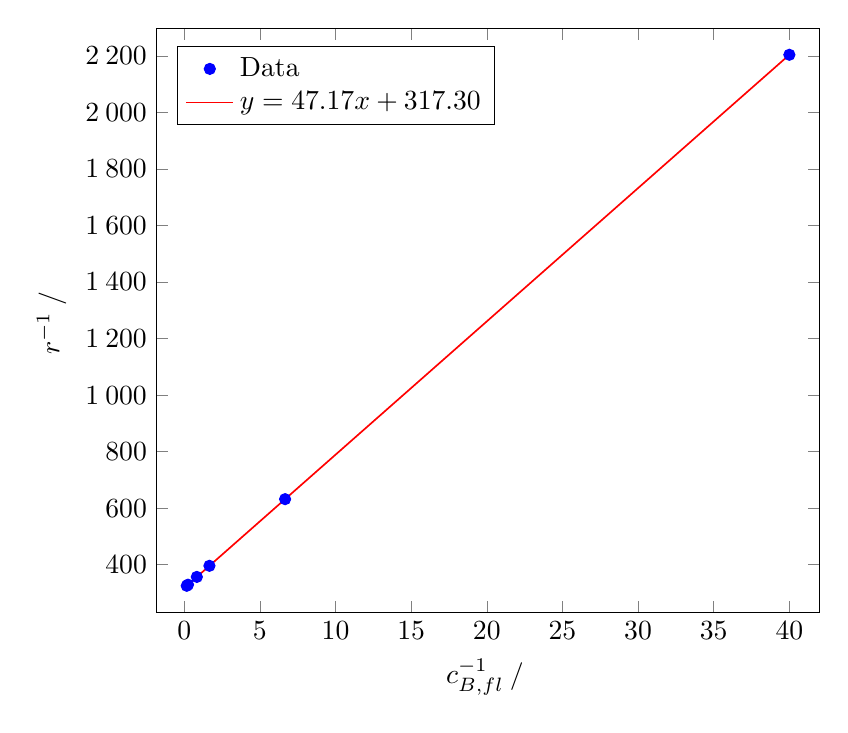
\begin{tikzpicture}
\begin{axis}[
height=9cm,
legend cell align={left},
legend pos=north west,
width=10cm,
xlabel={$ c_{B,fl}^{-1}\: / \: \si{\liter\per\mole}$},
xmin=-1.825, xmax=41.9916666666667,
ylabel={$r^{-1}\: / \: \si{\liter\second\per\mole}$},
ymin=231.206530949541, ymax=2298.21657434581,
]
\addplot [draw=blue, fill=blue, mark=*, only marks]
table{%
x  y
40 2204.26157237326
6.66666666666667 631.778456354638
1.66666666666667 395.908940943583
0.833333333333333 356.612184249629
0.25 329.109758104328
0.166666666666667 325.168003468459
};
\addlegendentry{Data}
\addplot [semithick, red]
table {%
40 2204.25883169654
6.66666666666667 631.792472889477
1.66666666666667 395.922519068417
0.833333333333333 356.61086009824
0.25 329.092698819116
0.166666666666667 325.161532922099
};
\addlegendentry{$y=47.17x+317.30$}
\end{axis}
\end{tikzpicture}

\end{center}
%%
The rate constant $k$ can be calculated by ($[m] = \si{second}$):
%%
\begin{equation}
 k = \frac{1}{m * H_A * p_A} = \pySI{k}{\liter\per\mole\second}
\end{equation}
%%
The product of the specific interface and the mass transport coefficient $a * \beta_L$ can be calculated by ($[d] = \si{\liter\second\per\mole}$):
%%
\begingroup 
\sisetup{round-precision=4}
\begin{equation}
 a * \beta_L = \frac{1}{d * H_A * p_A} = \pySI{aBetaL}{\per\second}
\end{equation}
\endgroup

%%
The concentration of the gas A in the liquid can by rearranging the mass balance $ \dot{n}_{diff} = \dot{n}_{rxn}$:
%%
\begin{align}
\begin{split}
&a * \beta_L * V_{fl} * \left( H_A * p_A - c_{A,fl}\right) = k * V_{fl} * c_{A,fl} * c_{B,fl}\\
&\Longrightarrow c_{A,fl} = \frac{a * \beta_L}{a * \beta_L + k * c_{B,fl}} * p_A * H_A
\end{split}
\end{align}
%%
The concentration of A in liquid without a further reaction can be calculated by rearranging the mass balance $\dot{n}_{diff} = 0$:
%%
\begin{align}
\begin{split}
&a * \beta_L * V_{fl} * \left( H_A * p_A - c_{A,fl}\right) = 0\\
&\Longrightarrow c_{A,fl} = H_A * p_A = \pySI{cAflwr}{\mole\per\liter}
\end{split}
\end{align}
%%
In the case of a high concentration of B $(k * c_{B,fl} \gg a * \beta_L)$ Eq. \ref{eqn8:rate} simplifies to:
%%
\begin{equation}
 r = k * a * \beta_L * H_A * p_A
\end{equation}
%%
\end{solution}


